For part one of this lab, a simple Array Helper library written in Java was
tested using mutation testing. A Java library named PIT test was used to 
generate mutants of the ArrayLib class. Test cases were created which had 100\%
line coverage and branch coverage. These are outlined in the table which can be found in Appendix \ref{part1table}
The failing tests are explained as follows:

\begin{enumerate}
\item \underline{withoutTestRemoveTwo}:
        This test fails because this method depends on ArrayLib's implementation
        of indexOf, which only returns the first occurrence of an element. This
        results in the method only removing one occurrence of a repeated
        element.
\item \underline{withoutTestRemoveFirstElement}:
        This test fails because in the method, there is a check to see if
        $index > 0$, but it should be $index \geq 0$. Because it strictly checks
        for $index > 0$, the first element is never considered for removal.
\item \underline{intersectionTestDuplicate}:
        This test fails because if there are elements that appear more than once
        in both arrays, then the method will attempt to increment the index
        of the intersection array multiple times. However, this array is
        currently limited to the length of array a. To avoid this error, the
        size of the intersection array should be the length of array a plus the
        length of array b. 
\end{enumerate}

To do the mutation testing, the three failing tests above were commented out,
since mutation testing has a prerequisite, which is that the test suite must be
green. With the PIT tool, 37 mutants were created, and 36 were killed. (More on
this later).

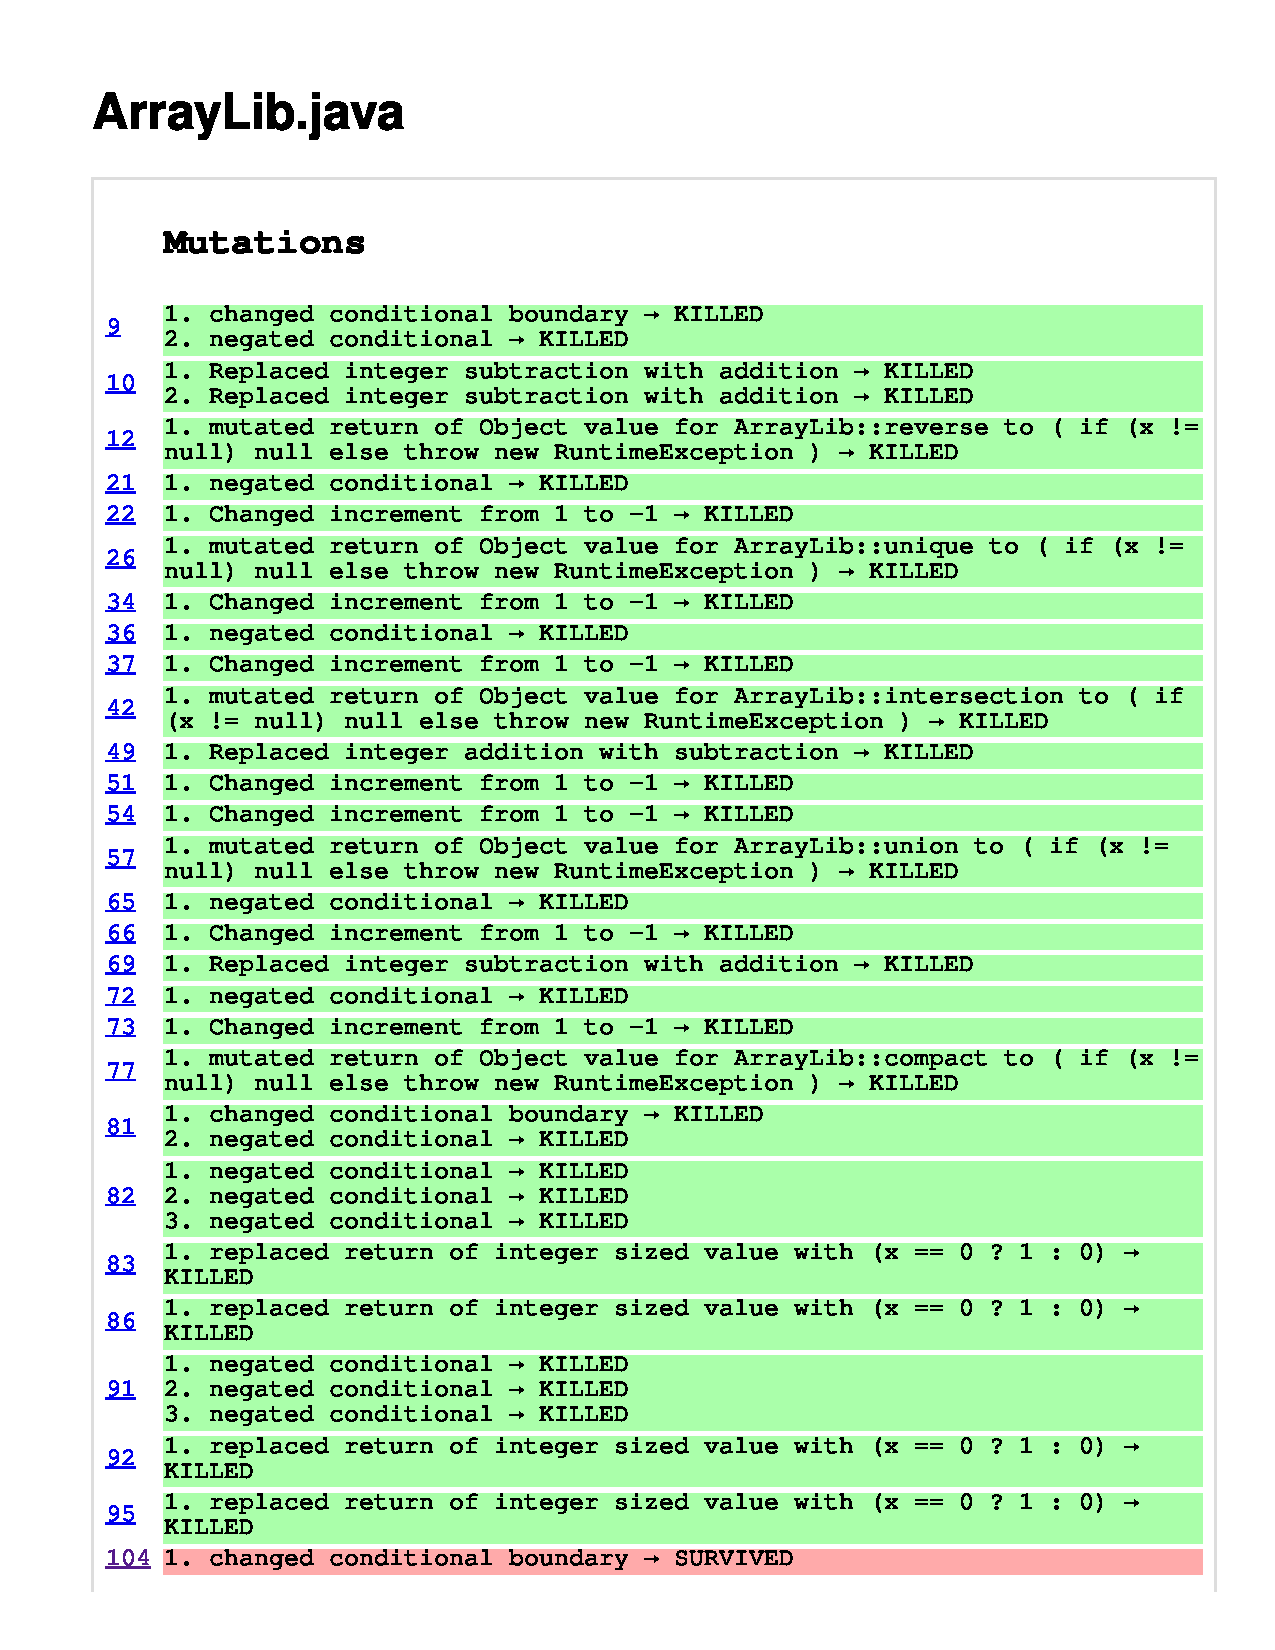
\includepdf[pages=-]{resources/pitest.pdf}

Now, for the one mutant that survived, it is actually directly related to a test
failure mentioned above, which we commented out before running PITest.
Specifically, it has to do with the if statement which checks if $index > 0$
instead of $index \geq 0$ on line 104. 


Before the mutation testing, we found three bugs in the program. After the
mutants were created and killed, only one of the bugs was highlighted. By the
mutation test report. In this case, the mutation testing did not expose holes in
the succeeding test cases, but this was mostly due to the luck of the tester
writing good test cases. In other applications, mutation testing can and will
help find holes in weak test suites. This is reinforced by the fact that after
we commented out the failing tests, the mutation test caught one of the bugs
because a mutant survived when the condition on line 104 $index > 0$ was mutated.

I think in the real world mutation testing can be used as an indicator, a sort
of `litmus' test, if you will for the quality of a test suite. It by no means
should be the only thing one checks for to evaluate the quality of a testing
suite, but on its own, it can reveal some weaknesses in a test suite. Like any
other testing strategy, it is not a silver bullet, and the right testing
strategies should be used for the right situations. In general, mutation testing
excels at checking boundary conditions, which can be extremely useful, since
programmers often mix up conditions such as `less than' or `less than or equal
to'.
